\begin{frame}{wifi modes}
    \begin{itemize}
    \item ``ad-hoc'': everyone sends/receives from whoever
    \item ``infrastructure'': designated \textit{access points}
    \vspace{.5cm}
    \item mostly use infrastructure networks
    \end{itemize}
\end{frame}

\begin{frame}{infrastructure mode}
    \begin{itemize}
    \item networks identified by SSID (Service Set IDentifier)
        \begin{itemize}
        \item human readable name
        \end{itemize}
    \item single SSID can have many access points (example: eduroam)
    \item clients \textit{associated} with one access point at a time
    \vspace{.5cm}
    \item clients only \textit{only} send to their current access point
    \item \ldots even if sending to other nodes on network
    \end{itemize}
\end{frame}

\begin{frame}{exercise: why through AP?}
    \begin{itemize}
    \item case where going through AP helps performance?
    \item case where going through AP hurts performance?
    \end{itemize}
\end{frame}

\begin{frame}{beacons (approx. once per 100ms)}
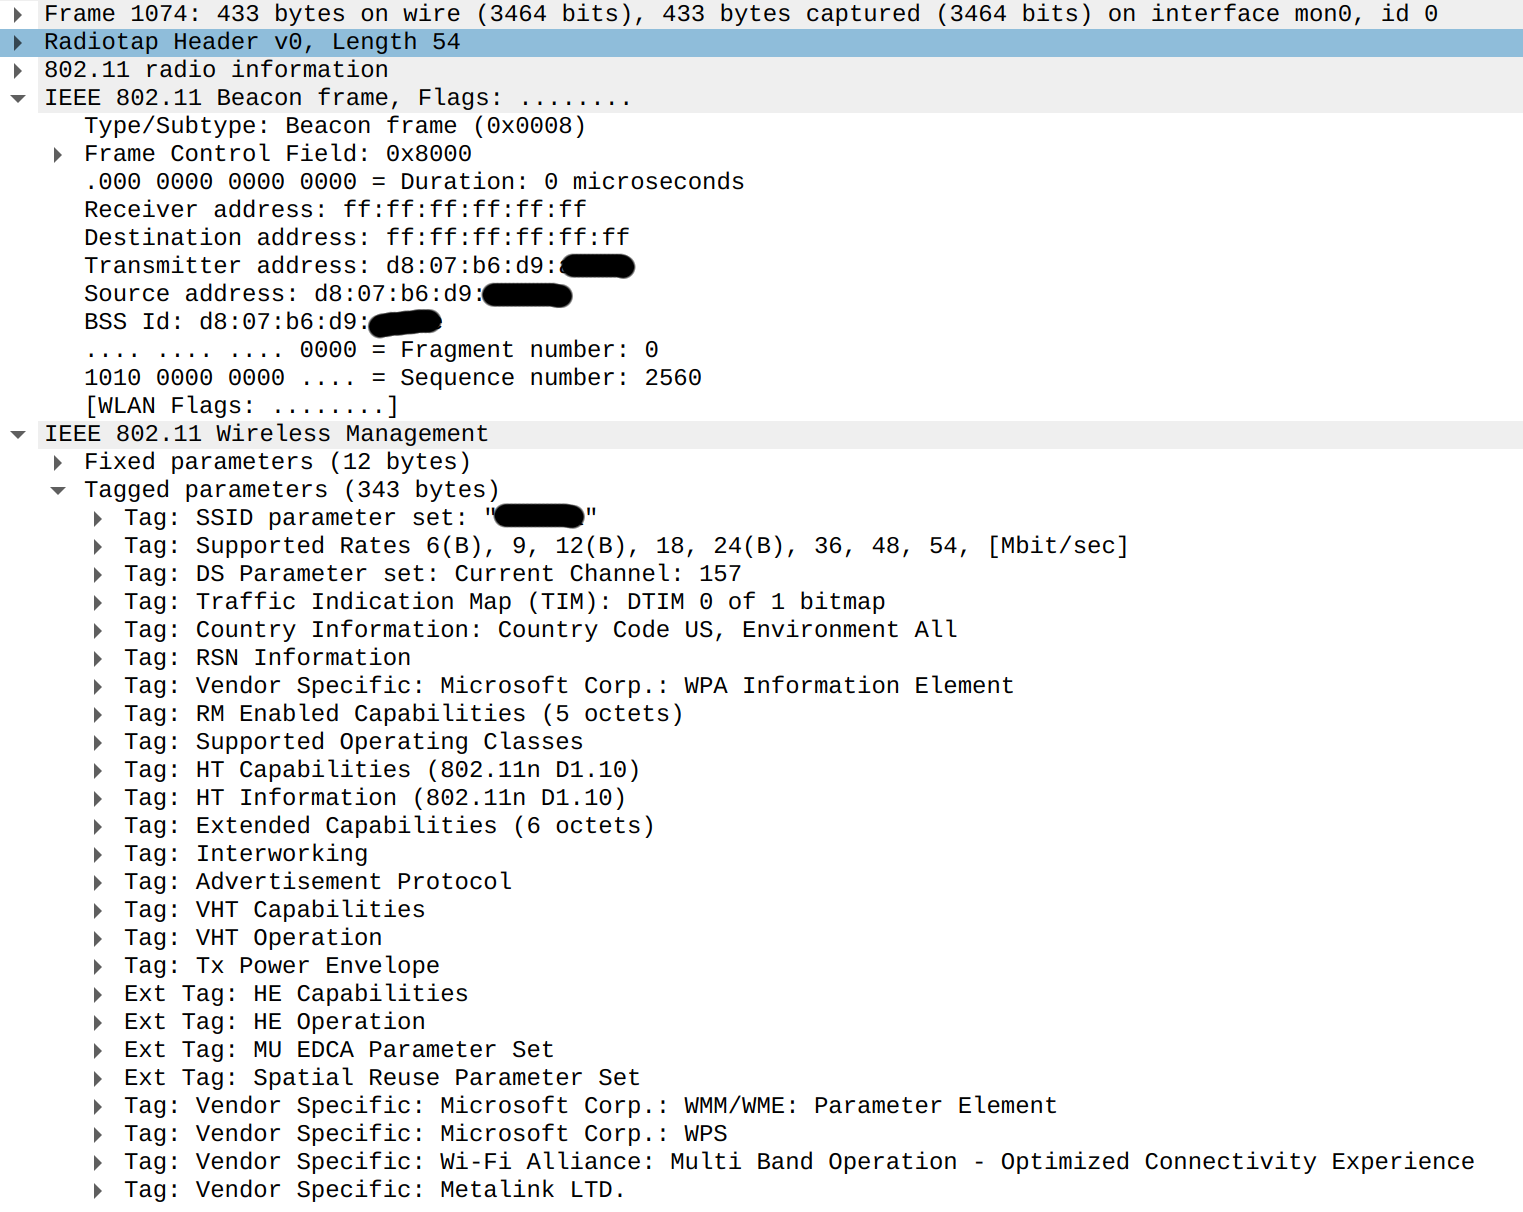
\includegraphics[height=0.85\textheight]{../multiaccess/wifi-beacon-1.png}
\end{frame}

\begin{frame}{probes/probe responses}
    \begin{itemize}
    \item beacons --- listen for a few seconds, find out about nearby networks
    \item probably need to scan multiple channels
    \vspace{.5cm}
    \item can also send explicit probes to learn about networks
    \item receive responses, with essentially same kind of information
    \end{itemize}
\end{frame}

\begin{frame}{association}
    \begin{itemize}
    \item client $\rightarrow$ AP: association response (SSID=\ldots)
    \item AP $\rightarrow$ client: association response (SSID=\ldots)
    \item + things related to WiFi Security (encryption, passwords, etc.)
    \vspace{.5cm}
    \item client $\rightarrow$ AP: deassociation (sometimes)
    \end{itemize}
\end{frame}

\begin{frame}{moving between APs}
    \begin{itemize}
    \item multiple APs can broadcast have same SSID
    \item generally: nodes should listen for beacons, measure signal-to-noise ratio
    \vspace{.5cm}
    \item eventually decide to change association
    \end{itemize}
\end{frame}


\begin{frame}{wifi data frames}
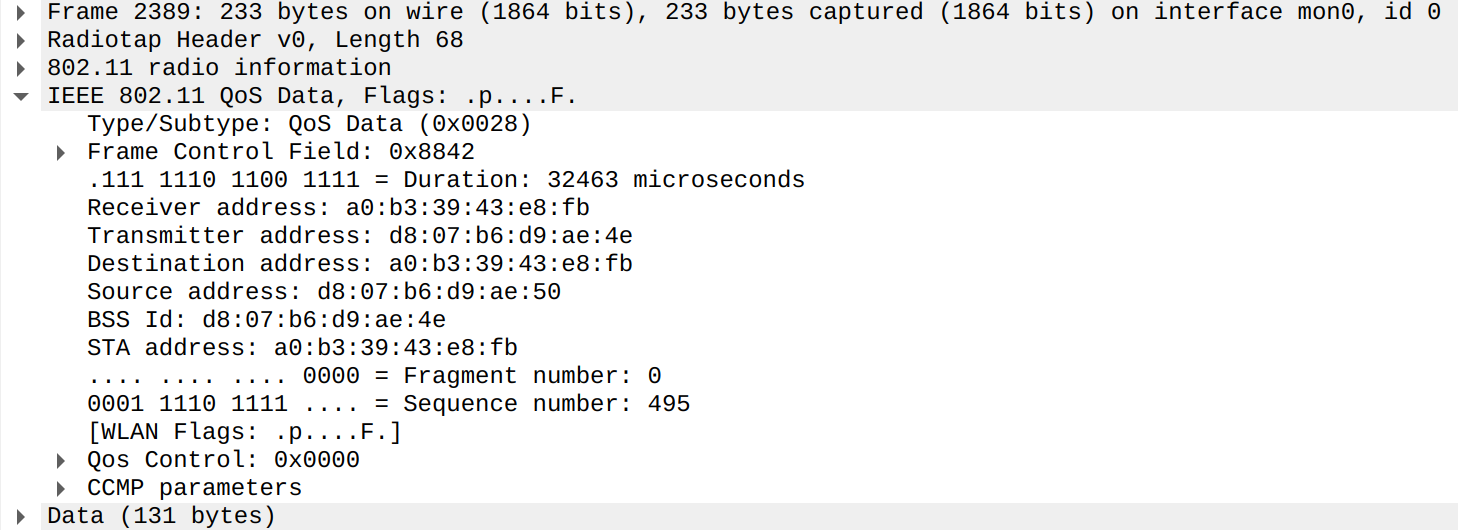
\includegraphics[height=0.85\textheight]{../multiaccess/wifi-data-1.png}
\end{frame}

\begin{frame}{wifi data}
\begin{tikzpicture}
\node (A) at (0, 0) {A};
\node (ap1) at (4, 0) {AP1};
\node (ap2) at (8, 0) {AP2};
\node (B) at (12, 0) {B};
\begin{scope}[-Latex]
\draw (A) -- (ap1);
\draw (ap1) -- (ap2);
\draw (ap2) -- (B);
\end{scope}
\end{tikzpicture}
    \begin{itemize}
    \item receiver/transmitter address --- this hop
    \item source/destination address --- final soruce/destination
    \vspace{.5cm}
    \item can differ if\ldots
        \begin{itemize}
        \item destination is a broadcast/multicast address
        \item wireless equivalent of `switching'
        \end{itemize}
    \end{itemize}
\end{frame}

